\documentclass[a4paper,11pt]{article}

% 日本語対応
\usepackage{xeCJK}
\setCJKmainfont{Yu Gothic}

% 数学関連パッケージ
\usepackage{amsmath}
\usepackage{amssymb}
\usepackage{amsthm}
\usepackage{amsfonts}
\usepackage{mathtools}

% 図形描画用パッケージ
\usepackage{tikz}
\usepackage{pgfplots}
\pgfplotsset{compat=1.18}

% その他パッケージ
\usepackage{graphicx}
\usepackage{enumitem}
\usepackage{float}
\usepackage{hyperref}
\usepackage{fancyhdr}
\usepackage{geometry}

% ページ設定
\geometry{
  a4paper,
  top=25mm,
  bottom=25mm,
  left=25mm,
  right=25mm
}

% ヘッダーとフッターの設定
\pagestyle{fancy}
\fancyhf{}
\fancyhead[L]{数学問題(選択式)}
\fancyhead[R]{\today}
\fancyfoot[C]{\thepage}
\renewcommand{\headrulewidth}{0.4pt}
\renewcommand{\footrulewidth}{0.4pt}

% タイトル情報
\title{数学問題(選択式)}
\author{数学問題生成AIシステム}
\date{\today}

% 選択肢スタイルの設定
\newcommand{\choice}[2]{
    \item[#1)] #2
}

% ドキュメント開始
\begin{document}

\maketitle

% 問題セクション
\section*{問題}

% 問題文を挿入(変数で置換)
次の二次方程式 $x^2 - 6x + 8 = 0$ の解として正しいものを選びなさい。

% 選択肢を挿入
\begin{description}[labelwidth=1cm, leftmargin=!]
\choice{A}{$x = -2, x = -4$}
\choice{B}{$x = -2, x = 4$}
\choice{C}{$x = 2, x = 4$}
\choice{D}{$x = 1, x = 8$}
\end{description}

% 解答セクション(オプショナル - 表示したくない場合はコメントアウト)
\section*{解答}

% 解答を挿入(変数で置換)
正解は C) $x = 2, x = 4$ です。

% 解説セクション(オプショナル - 表示したくない場合はコメントアウト)
\section*{解説}

% 解説を挿入(変数で置換)
$x^2 - 6x + 8 = 0$ を因数分解すると $(x - 2)(x - 4) = 0$ となる。
したがって、$x = 2$ または $x = 4$ が解である。

% 図形が必要な場合はここに挿入
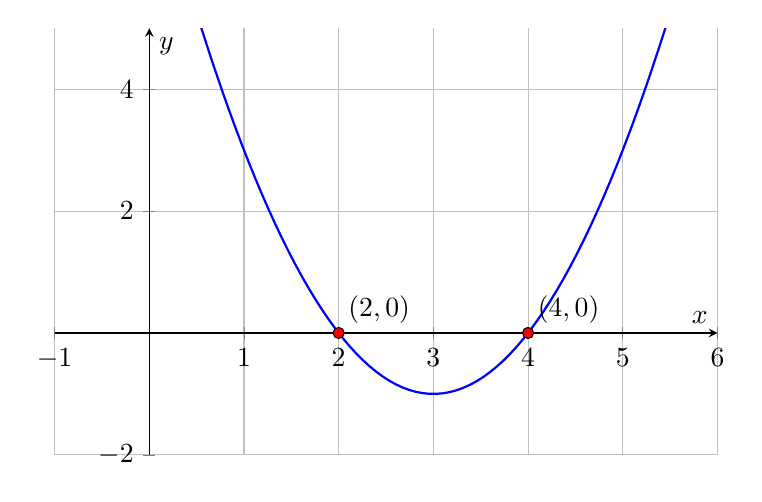
\begin{tikzpicture}
        \begin{axis}[
          axis lines=middle,
          xlabel=$x$,
          ylabel=$y$,
          xmin=-1, xmax=6,
          ymin=-2, ymax=5,
          grid=both,
          width=10cm,
          height=7cm
        ]
          \addplot[domain=-1:6, samples=100, blue, thick] {x^2 - 6*x + 8};
          \addplot[mark=*, fill=red] coordinates {(2,0)} node[above right] {$(2,0)$};
          \addplot[mark=*, fill=red] coordinates {(4,0)} node[above right] {$(4,0)$};
        \end{axis}
      \end{tikzpicture}

\end{document} 